\documentclass{amsart}
\usepackage{amsmath, amsfonts, amssymb}
\usepackage{tikz-cd}
\usepackage{bm}
\usepackage[boxruled, noend]{algorithm2e}
\usepackage{graphicx, fancyvrb}

% hyperref
\usepackage[bookmarks=true,
bookmarksnumbered=true, breaklinks=true,
pdfstartview=FitH, hyperfigures=true,
plainpages=false, naturalnames=true,
colorlinks=true, pagebackref=true,
pdfpagelabels]{hyperref}
\hypersetup{
	linktocpage,
	colorlinks,
	citecolor=blue,
	linkcolor=blue,
	urlcolor=blue}

% layout
\setlength{\textwidth}{\paperwidth}
\addtolength{\textwidth}{-1.5in}
\setlength{\textheight}{\paperheight}
\addtolength{\textheight}{-2in}
\calclayout

% update to MSC2020
\makeatletter
\@namedef{subjclassname@2020}{%
	\textup{2020} Mathematics Subject Classification}
\makeatother

\newcommand{\W}{\mathsf{W}}
\newcommand{\F}{\mathbb{F}}
\renewcommand{\S}{\mathrm{S}}
\renewcommand{\k}{\Bbbk}
\renewcommand{\th}{\mathrm{th}}
\DeclareMathOperator{\xor}{\triangle}
\DeclareMathOperator{\eval}{eval}
\DeclareMathOperator{\pos}{pos}
\newcommand{\bu}{{\bar{u}}}
\newcommand{\sm}{\smallsetminus}
\newcommand{\R}{\mathbb{R}}
\newcommand{\RP}{\mathbb{R}\mathrm{P}}
\newcommand{\suspension}{\Sigma}

\newcommand{\Z}{\mathbb{Z}}
\renewcommand{\P}{\mathrm{P}}
\newcommand{\D}{\mathrm{D}}
\newcommand{\chains}{C_\bullet}
\newcommand{\cochains}{C^\bullet}
\newcommand{\Hom}{\mathrm{Hom}}
\newcommand{\Mod}{\mathbf{Mod}_{\F}}
\newcommand{\cMod}{\mathbf{Mod}_{\F}^{\simplex}}
\newcommand{\Ch}{\mathbf{Ch}_{\F}}
\newcommand{\cCh}{\mathbf{Ch}_{\F}^{\simplex}}
\newcommand{\sSet}{\mathbf{sSet}}
\newcommand{\id}{\mathrm{id}}
\newcommand{\ind}{\mathrm{ind}}
\newcommand{\p}{\mathrm{p}}
\newcommand{\q}{\mathrm{q}}
\newcommand{\Sq}{\mathrm{Sq}}
\newcommand{\simplex}{\bm{\Delta}}

\DeclareMathOperator*{\displaytensor}{\otimes}

% environment
\newtheorem{theorem}{Theorem}
\newtheorem{proposition}[theorem]{Proposition}
\newtheorem{lemma}[theorem]{Lemma}
\newtheorem{corollary}[theorem]{Corollary}
\newtheorem{claim}[theorem]{Claim}
\theoremstyle{definition}
\newtheorem{definition}[theorem]{Definition}
\newtheorem{example}[theorem]{Example}
\newtheorem{remark}[theorem]{Remark}
\newenvironment{tab}{\list{}{\rightmargin 0pt}\item\relax}{\endlist}

% other
\newcommand{\anibal}[1]{\textcolor{blue}{\underline{Anibal}: #1}}
\renewcommand{\th}{^\mathrm{th}}

\begin{document}	
	\title{New formulas for the cup-$i$ products and fast computation of Steenrod squares}
	\author{Anibal M. Medina-Mardones}
	\thanks{...}
	\address{Department of Mathematics, University of Notre Dame}
	\email{amedinam@nd.edu}
	
	\begin{abstract}
		We present new formulas for cup-$i$ products on the singular cochains of spaces and use them to introduce a fast algorithm for the computation of Steenrod squares on simplicial cohomology of simplicial complex.
	\end{abstract}
	
	\maketitle
	\tableofcontents	
	
\section{Introduction}

For effective computations involving topological spaces, discrete models are indispensable.
The category of simplicial complexes provides models not only for spaces but also, through the simplicial approximation theorem, for continuous maps between them.
We can obtain from these combinatorial models algebraic ones using the simplicial chains construction $\chains$.
In this algebraic representation, invariants of spaces such as their betti numbers ---the ranks of its cohomology with field coefficients--- can be readily computed through linear algebra alone.

In this article we focused on finer invariants of spaces enriching their mod 2 cohomology and going beyond betti numbers.
We are referring to the celebrated Steenrod squares
\begin{equation*}
Sq^k \colon H^\bullet(X; \F_2) \to H^\bullet(X; \F_2)
\end{equation*}
which can be thought of as arising from the broken $\S_2$-symmetry of the diagonal map
\begin{equation*}
\begin{tikzcd}[column sep=small, row sep=tiny]
X \arrow[r] & X \times X \\
x \arrow[r, mapsto] & (x,x)
\end{tikzcd}
\end{equation*}
occurring during the passage from continuous objects to discrete/algebraic models.

For simplicial complexes, effective constructions of Steenrod squares have been known since their introduction in Steenrod's seminal 1947 paper \cite{steenrod47}.
They all rely on the construction of \textit{cup-$i$ coproducts}
\begin{equation*}
\Delta_i \colon \chains(X; \F_2)  \to \chains(X; \F_2)^{\otimes 2}\,,
\end{equation*}
natural linear maps satisfying $\Delta_i = 0$ for $i < 0$ and
\begin{equation} \label{e:boundary of cup-i}
(1 + T) \Delta_{i-1} = \partial \circ \Delta_i + \Delta_i \circ \partial,
\end{equation}
with $\Delta_0$ a chain approximation to the diagonal of $X$.
The linear dual maps on cochains
\begin{equation*}
\smallsmile_i \colon \cochains(X; \F_2)^{\otimes 2} \to \cochains(X; \F_2).
\end{equation*}
are known as \textit{cup-$i$ products}.

Several constructions of cup-$i$ coproducts have been given in the literature starting with Steenrod's original formulas.
These include the approach of Real \cite{real1996computability} and Gonz\'alez-D\'iaz--Real \cite{gonzalez1999combinatorial, gonzalez2003computation, gonzalez2005hpt} based on the EZ-AW chain contraction, the operadic constructions of McClure-Smith \cite{mcclure03cochain} and Berger-Fresse \cite{berger04combinatorial}, and the prop approach of the author \cite{medina2020prop1, medina2018prop2}.
Although it has been surprisingly shown \cite{medina2018axiomatic} that all of these define isomorphic cup-$i$ coproducts, the alternative descriptions are better suited for different tasks.
For effective computations of Steenrod squares on simplicial complexes, and algorithm based on \cite{gonzalez1999combinatorial} was implemented in the open-source mathematics system \verb|SAGE| by John Palmieri \cite{sagemath}.

In this article we introduce a new description of Steenrod's cup-$i$ coproducts which is in a sense dual to his.
We are particularly interested in simplicial complexes, but we remark that our formulas apply to the more general context of simplicial sets, a categorical closure of simplicial complexes that include as examples the singular cochains of any topological space.
For simplicial complexes we use our formulas to introduce a new algorithm computing Steenrod squares, and loosely test it performance implemented in \verb|Python| against the one in \verb|SAGE|.

The speed gained with our algorithm is essential for the incorporation of Steenrod squares into persistence homology \cite{medina2018persistence}, a technique typically used in highly intensive data analysis tasks, for example \cite{chan2013topology, lee2018nanoporous}, and for which various softwares have been developed, including \cite{bauer2019ripser, gudhi, medina2020giottotda}.

On the theoretical side, our formulas can serve as a template for the definition of mod 2 cohomology operations in other contexts.
For example, Cantero-Mor\'an \cite{cantero2020khovanov} followed this approach to define Steenrod squares in Khovanov homology.

Other areas besides topology where cup-$i$ products have become important are:condensed matter physics, where they are used to describe action functionals of discrete topological field theories \cite{gaiotto2016spin, bhardwaj2017state, kapustin2017fermionic}, higher category theory, where they can be used to deduce the nerve of $\omega$-categories \cite{medina2020globular}, and convex geometry, where they are connected to projections of cyclic polytopes \cite{kapranov1991combinatorial}.
It is our hope that the new description of cup-$i$ products presented in this article can serve to facilitate new connections to deepen those already established.

In Section~\ref{s:preliminaries} we review the notions from equivariant homological algebra and simplicial topology needed to present, in Section~\ref{s:squares}, a definition of Steenrod squares in terms of cup-$i$ products.
We introduce our new formulas in Section~\ref{s:formulas}, and our algorithm for the computation of Steenrod squares in Section~\ref{s:algorithm}; providing a proof-of-concept comparison using \verb|SAGE| in Section~\ref{s:comparison}.
In Section~\ref{s:proof} we prove that our new formulas define cup-$i$ coproducts, and in Section~\ref{s:outlook} we present an outlook of future research directions.
	
\subsection*{Acknowledgments} We would like to thank Dennis Sullivan, Kathryn Hess, Stephan Stolz, Mark Behrens, John Morgan, Greg Brumfiel, Federico Cantero Mor\'an, Tim Campion, and Riley Levy for their insights, questions, and comments about this project.
	%!TEX root = ../fast_sq.tex

\section{Preliminaries} \label{s:preliminaries}

In this section we review the basic notions used in this article and set up the conventions we follow.

\subsection{Chain complexes}

We assume familiarity with the notion of chain complex over a ring $\k$.

The \textit{tensor product} $C \otimes C^\prime$ of chain complexes $C$ and $C^\prime$ is the chain complex whose degree-$n$ part is
\begin{equation*}
\left(C \otimes C^\prime\right)_n = \bigoplus_{i+j=n} C_i \otimes C^\prime_j,
\end{equation*}
where $C_i \otimes C^\prime_j$ is the tensor product of $\k$-modules, and whose boundary map is defined by
\begin{equation*}
\partial (v \otimes w) = \partial v \otimes w + (-1)^{|v|} v \otimes \partial w.
\end{equation*}

The \textit{hom complex} $\Hom(C, C^\prime)$ is the chain complex whose degree-$n$ part is the subset of linear maps between them that shift degree by $n$, i.e.,
\begin{equation*}
\Hom(C, C^\prime)_n = \{f \mid f(C_k) \subseteq C^\prime_{k+n}\},
\end{equation*}
and boundary map defined by
\begin{equation*}
\partial f = \partial_{C^\prime} \circ f - (-1)^{n} f \circ \partial_C.
\end{equation*}
Notice that a chain map is the same as a $0$-cycle in this complex, and that two chain maps are chain homotopy equivalent if and only if they are homologous cycles.
We extend this terminology and say that two maps $f, g \in \Hom(C, C^\prime)$ are \textit{homotopic} if their difference is nullhomologous, referring to a map $h \in \Hom(C, C^\prime)$ such that $\partial h = f - g$ as a \textit{homotopy} between $f$ and $g$.

Regarding $\k$ as a chain complex concentrated in degree $0$, the \textit{linear dual} of a chain complex $C$ is the chain complex $\Hom(C, \k)$.
We refer to the contravariant functor $\Hom(-, \k)$ as \textit{linear duality}.

For any three chain complexes, there is a natural isomorphism of chain complexes
\begin{equation} \label{e:adjunction isomorphism}
\Hom(C \otimes C^\prime, C^{\prime\prime}) \cong
\Hom(C, \Hom(C^\prime, C^{\prime\prime}))
\end{equation}
referred to as the \textit{adjunction isomorphism}.

\subsection{Group actions}

Symmetries on chain complexes play an important role on this work.
Let $G$ be a finite group.
We will later focus solely on the symmetric group $\Sym_2$.
We denote by $\k[G]$ the group ring of $G$, i.e., the free $\k$-module generated by $G$ together with the ring product defined by linearly extending the product in $G$.
We refer to a chain complex of left $\k[G]$-modules as a chain complex with a $G$-\textit{action} and to $\k[G]$-linear maps as $G$-\textit{equivariant}.

Given a chain complex $C$ with a $G$-action we naturally associate the following two chain complexes.
The subcomplex of \textit{invariant chains} of $C$, denoted $C^G$, contains all elements $c \in C$ satisfying $g \cdot c = c$ for every $g \in G$.
The quotient complex of \textit{coinvariant chains} of $C$, denoted $C_G$, is the chain complex obtained by identifying elements $c, c^\prime \in C$ if there exists $g \in G$ such that $c^\prime = g \cdot c$.

Let $C$ and $C^\prime$ be chain complexes and assume $C$ has a $G$-action.
The chain complex $\Hom(C, C^\prime)$ has a $G$-action induced from $(g \cdot f)(c) = f^{-1}(g^{-1} \cdot c)$ and there is an isomorphism
\begin{equation} \label{e:invariant hom iso hom coinvariants}
\Hom(C, C^\prime)^G \cong \Hom(C_G, C^\prime).
\end{equation}

\subsection{Simplicial topology}

Simplicial complexes are used to combinatorially encode the topology of spaces.
An \textit{abstract and ordered simplicial complex}, or a \textit{simplicial complex} for short, is a pair $(V, X)$ with $V$ a poset and $X$ a set of subsets of $V$ such that:
\begin{enumerate}
	\item The restriction of the partial order of $V$ to any element in $X$ defines a total order on it.
	\item For every $v$ in $V$, the singleton $\{v\}$ is in $X$.
	\item If $x$ is in $X$ and $y$ is a subset of $x$, then $y$ is in $X$.
\end{enumerate}
We abuse notation and denote the pair $(V, X)$ simply by $X$ referring to $V$ as its poset of vertices.

The elements of $X$ are called \textit{simplices} and the \textit{dimension} of a simplex $x$ is defined by subtracting $1$ from the number of vertices it contains.
Simplices of dimension $n$ are called $n$-simplices and are denoted by their order set of vertices $[v_0, \dots, v_n]$.
The collection of $n$-simplices of $X$ is denoted $X_n$.
There are natural maps $d_i^n \colon X_n \to X_{n-1}$ for $i \in \{0, \dots, n\}$ defined by
\begin{equation*}
d_i^n([v_0, \dots, v_n]) = [v_0, \dots, \widehat{v}_i, \dots, v_n]
\end{equation*}
and referred to as the $i^\th$ face map in dimension $n$.
These satisfy the \textit{simplicial relation}:
\begin{equation} \label{e:simplicial relation}
d_i^{n-1} d^n_j = d_{j-1}^{n-1} d_i^n
\end{equation}
for any $0 \leq i < j \leq n$.
We will omit the superscripts of these maps when no confusion arises from doing so.

A \textit{simplicial map} $X \to X^\prime$ is a morphisms between their posets of vertices $f \colon V \to V^\prime$ sending simplices to simplices, i.e., satisfying that if $[v_0, \dots, v_n] \in X$ then $[f(v_0), \dots, f(v_n)] \in X^\prime$.

Let $X$ be simplicial complex.
The degree-$n$ part of the chain complex of \textit{chains} of $X$, which we denote $C_\bullet(X; \k)$, is defined by
\begin{equation*}
C_n(X; \k) = \k \big\{ X_n \big\},
\end{equation*}
i.e., the $\k$-module freely generated by the $n$-dimensional simplices of $X$.
The boundary map is defined on simplices by
\begin{equation*}
\begin{tikzcd}[column sep=normal, row sep=tiny,row sep = 0ex
,/tikz/column 1/.append style={anchor=base east}
,/tikz/column 2/.append style={anchor=base west}
]
C_n(X; \k) \arrow[r, "\partial_n"] & C_{n-1}(X; \k) \\
x\ \arrow[r, |->] & \sum_{i=0}^{n} (-1)^i d_i (x).
\end{tikzcd}
\end{equation*}

Given a simplicial map $f \colon X \to X^\prime$, the \textit{induced chain map} $f_\bullet \colon C_\bullet(X; \k) \to \chains(X^\prime; \k)$ is defined on simplices by $f_\bullet([v_0, \dots, v_n]) = [f(v_0), \dots, f(v_n)]$ if $i \neq j$ implies $ f(v_i) \neq f(v_j)$ and it is $0$ otherwise.

We refer to
\begin{equation*}
C^\bullet(X; \k) = \Hom \big( C_\bullet(X; \k), \k \big)
\end{equation*}
as the \textit{cochains} of $X$ and to the dual $\delta^{n}$ of $\partial_{-n}$ as the $n^\th$ coboundary map.
Furthermore, we denote the linear dual of the map $f_\bullet$ induced by a simplicial map $f$ by $f^\bullet$.
We remark that $C_n(X; \k) = 0$ for $n < 0$ and $C^n(X;\k) = 0$ for $n > 0$.
Elements in the kernel of $\delta_n$ are called \textit{cocycles} and those in the image of $\delta_{n+1}$ \textit{coboundaries}.
The $n^\th$-\textit{cohomology} $H^n(X; \k)$ of $X$ is the quotient $\ker \delta_n / \img \delta_{n+1}$.
We denote by $[\alpha]$ the cohomology class represented by a cocycle $\alpha$.

We will abuse notation and identify simplices in $X_n$ with their associated basis elements in $\chain{n}(X; \k)$, and when $X$ and $\k$ are clear from the context we will omit them.
	%!TEX root = ../fast_sq.tex

\section{Cup-\texorpdfstring{$i$}{i} constructions and Steenrod squares} \label{s:squares}

Let $\Ftwo$ be the field with two elements and $\Sym_2$ the group with only one non-identity element $T$.
In this section we define for any simplicial complex $X$ and every integer $k$ the $k^\th$ Steenrod square
\begin{equation*}
Sq^k \colon H^\bullet(X; \Ftwo) \to H^{\bullet}(X; \Ftwo)
\end{equation*}
using an arbitrary cup-$i$ construction.

\subsection{Cup-$i$ constructions}

Consider the chain complex
\begin{equation*}
\begin{tikzcd}[column sep=normal]
& W =  \Ftwo[\Sym_2]\{e_0\} & \arrow[l, "1+T"'] \Ftwo[\Sym_2]\{e_1\} & \arrow[l, "1+T"']
\Ftwo[\Sym_2]\{e_2\} & \arrow[l, "1+T"'] \cdots
\end{tikzcd}
\end{equation*}
with its natural $\Sym_2$-action.
For any simplicial complex $X$, the chain complex $W \otimes C_\bullet(X; \Ftwo)$ has an $\Sym_2$-action concentrated on the left factor, and $C_\bullet(X; \Ftwo)^{\otimes 2}$ has one given by transposition of factors.

We are interested in $\Sym_2$-equivariant chain maps
\begin{equation} \label{e:steenrod diagonal}
\Delta_X \colon W \otimes C_\bullet(X; \Ftwo) \to C_\bullet(X; \Ftwo)^{\otimes 2}
\end{equation}
defined naturally for every simplicial complex $X$, i.e., such that $\Delta_Y \circ (\id_W \otimes f_\bullet) = (f_\bullet \otimes f_\bullet) \circ \Delta_X$ for any simplicial map $f \colon X \to Y$.

\begin{definition}
	A \textit{cup-$i$ construction} is a natural collection of maps as above such that $\Delta_X \neq 0$ if $X$ is a simplicial complex with a single vertex.
\end{definition}

A cup-$i$ construction is determined by a collection $\{\Delta_i\}_{i \in \Z}$ of natural linear maps $C_\bullet \to C_\bullet^{\otimes 2}$ satisfying $\Delta_0 \big([v]\big) \neq 0$ for any vertex $v$ and
\begin{equation} \label{e:boundary of cup-i}
(1 + T) \Delta_{i-1} = \partial \circ \Delta_i + \Delta_i \circ \partial
\end{equation}
for any $i \in \Z$.
The correspondence is given by $\Delta_i = \Delta(e_i \otimes -)$, and we refer to the map $\Delta_i$ as the \textit{cup-$i$ coproduct} of the cup-$i$ construction, and to the linear dual $\smallsmile_i$ of $\Delta_i$ as its \textit{cup-$i$ product}.
Explicitly, given two cochains $\alpha$ and $\beta$ and a chain $c$ we have
\begin{equation*}
(\alpha \smallsmile_i \beta)(c) = (\alpha \otimes \beta) \Delta_i(c).
\end{equation*}

\subsection{Steenrod squares}

Let us consider a cup-$i$ construction $W \otimes C_\bullet \to C_\bullet^{\otimes 2}$.
Using the linear duality functor and passing to fix points gives a chain map
\begin{equation*}
\begin{tikzcd}
\Hom\left(C_\bullet \otimes C_\bullet, \Ftwo \right)^{\Sym_2} \arrow[r] &
\Hom\left(W \otimes C_\bullet, \Ftwo \right)^{\Sym_2},
\end{tikzcd}
\end{equation*}
which we can complete, using isomorphisms \eqref{e:adjunction isomorphism} and \eqref{e:invariant hom iso hom coinvariants} of \cref{s:preliminaries}, to a commutative diagram
\begin{equation*}
\begin{tikzcd}
\Hom\left(C_\bullet \otimes C_\bullet, \Ftwo \right)^{\Sym_2} \arrow[r] &
\Hom\left(W \otimes C_\bullet, \Ftwo \right)^{\Sym_2} \arrow[d] \\
\left(C^\bullet \otimes C^\bullet\right)^{\Sym_2} \arrow[u]&
\Hom\left(W_{\Sym_2} \otimes C_\bullet, \Ftwo \right) \arrow[d] \\
C^\bullet \arrow[u, "doubleing"] \arrow[r, dashed]&
\Hom\left(W_{\Sym_2}, C^\bullet\right),
\end{tikzcd}
\end{equation*}
where the choice of coefficients ensures that the \textit{doubleing map} $\alpha \mapsto \alpha \otimes \alpha$ is linear.
Using the adjunction isomorphism, the dashed arrow defines a linear map
\begin{equation} \label{e:Steenrod squares parameterized}
\begin{tikzcd}[row sep=0pt, column sep = small]
C^\bullet \otimes W_{\Sym_2} \arrow[r] &[-10pt] C^\bullet \\
\alpha \otimes e_i \arrow[r, |->] & (\alpha \otimes \alpha)\Delta_i(-)
\end{tikzcd}
\end{equation}
descending to mod $2$ cohomology.
The Steenrod squares are defined by reindexing this map.
Explicitly,
\begin{definition} \label{d:steenrod squares}
	The \textit{$k^\th$ Steenrod square} is defined by
	\begin{equation} \label{e:steenrod squares}
	\begin{tikzcd}[row sep=0pt, column sep=tiny]
	Sq^k \colon H^{-n} \arrow[r] & H^{-n-k} \\
	\phantom{Sq^k \colon}{[\alpha]} \arrow[r, |->] & {\left[(\alpha \otimes \alpha)\Delta_{n-k}(-) \right]}.
	\end{tikzcd}
	\end{equation}
	for any cup-$i$ construction $\Delta$.
\end{definition}

\subsection{Additional comments}

\begin{remark}[Simplicial sets]
	For the interested reader we mention that a cup-$i$ construction also defines, through a well known categorical construction, natural cup-$i$ coproducts on the chains of simplicial sets \cite{friedman2012simplicial} and, consequently, Steenrod squares in their mod 2 cohomology.
\end{remark}

\begin{remark}[Cup product] \label{r:cup product}
	Although in this article we do not use the algebra structure on the mod~2 cohomology of spaces, we remark that the cup-$0$ product of a cup-$i$ construction represents these so-called \textit{cup product}.
	Explicitly, if $[\alpha], [\beta] \in H^\bullet$ then $[\alpha][\beta] = [\alpha \smallsmile_0 \beta]$, in particular, if $[\alpha]$ is of degree $-k$ then $Sq^k\big([\alpha]\big) = [\alpha] [\alpha]$, which motivates the term squares in the name of the $Sq^k$ operations.
\end{remark}

\begin{remark}[Odd primes]
	For the reader familiar with group homology, we remark that Steenrod squares are parameterized by classes on the mod $2$ homology of $\Sym_2$.
	Steenrod used this group homology viewpoint to non-constructively define operations on the mod $p$ cohomology of spaces \cite{steenrod1962cohomology} for any prime $p$.
	To define these constructively, analogues of the $\Delta_i$ maps for odd primes were introduced in \cite{medina2021maysteenrod} and implemented in \cite{medina2021computer}.
\end{remark}
	
\section{New formulas} \label{s:formulas}

Let $X$ be a simplicial complex and $x \in X_n$. For a set
\begin{equation*}
U = \{u_1 < \dots < u_r\} \subseteq \{0, \dots, n\}
\end{equation*}
we use the notation $d_U(x) = d_{u_1} \ldots\, d_{u_r}(x)$.

\begin{definition} \label{d:cup-i coproducts}	
	For a non-negative integer $i$, the \textit{cup-$i$ coproduct}
	\begin{equation*}
	\Delta_i : C_\bullet(X; \F) \to C(X; \F)^{\otimes 2}_\bullet
	\end{equation*}
	is the linear map defined on a basis element $x \in X_n$ by
	\begin{equation} \label{equation: simplicial cup-i coproducts}
	\Delta_i(x) = \sum_U d_{U^+}(x) \otimes d_{U^-}(x),
	\end{equation}
	where the sum is taken over all sets $U = \{u_1 < \cdots < u_{n-i}\}$ with $u_j \in \{0, \dots, n\}$ and
	\begin{equation*}
	U^+ = \{u_j \in U\ |\ u_j \equiv j \text{ mod } 2\}, \qquad
	U^- = \{u_j \in U\ |\ u_j \not\equiv j \text{ mod } 2\}.
	\end{equation*}
	For a negative integer $i$ we set $\Delta_i = 0$.
\end{definition}

\begin{lemma}
	This construction is natural with respect to simplicial maps.
	Explicitly, if $f$ is a simplicial map, then, for every $i \in \Z$,
	\begin{equation*}
	\Delta_i \circ f_\bullet = (f_\bullet \otimes f_\bullet) \circ \Delta_i.
	\end{equation*}
\end{lemma}

\begin{proof}
	content...
\end{proof}

\begin{theorem} \label{t:main}
	For any integer $i$,
	\begin{equation} \label{eq: cup-i coproducts boundary relation}
	\partial \circ \Delta_{i} + \Delta_{i+1} \circ \partial = (1 +T ) \Delta_{i-1}.
	\end{equation}
\end{theorem}

We devote Section~\ref{s:proof} to the proof of this theorem.

\begin{example}
	AW diagonal and $Sq^0$.
	
	...
\end{example}
	%!TEX root = ../fast_sq.tex

\section{New algorithm for Steenrod squares} \label{s:algorithm}

\begin{figure}[b]
	%!TEX root = ../fast_sq.tex

\begin{algorithm} [H]
	\KwIn{$A = \{a_1, \dots, a_m\} \subseteq X_n$}
	$B = \emptyset$\\
	\ForAll{$a_i\ \mathrm{and}\ a_j\ \mathrm{with}\ i < j$}
	{
		$a_{ij} = a_i \cup a_j$\\
		\If{$a_{ij} \in X_{n+k}$}
		{
			$\overline{a}_i = a_i \setminus a_j$\ ;\ \
			$\overline{a}_j = a_j \setminus a_i$\ ;\ \
			$\overline{a}_{ij} = \overline{a}_i \cup \overline{a}_j$ \\
			$\ind \colon \overline{a}_{ij} \to \{0,1\}$ \\
			\ForAll {$v \in \overline{a}_{ij}$}
			{
				$p = \mathrm{position\ of\ } v \mathrm{\ in\ } a_{ij}$\ ;\ \
				$\overline{p} = \mathrm{position\ of\ } v \mathrm{\ in\ } \overline{a}_{ij}$\\
				$\ind(v) = {p}\, +\, \overline{p}\ \ \mathrm{residue\ mod}\ 2$
			}
			\If{\hspace*{3pt}$\ind(\overline{a}_i) \xor \ind(\overline{a}_j)$ = $\{0,1\}$}
			{$B = B \xor \, \{a_{ij}\}$}
		}
	}
	\KwOut{$B \subseteq X_{n+k}$}
	\caption{$SQ^k_n$}
	\label{a:algorithm}
\end{algorithm}
	\caption{Let $X$ be a simplicial complex $X$.
		Passing the support $A \subseteq X_n$ of a cocycle $\alpha$ and an integer $k \in \{1, \dots, n\}$, the algorithm returns the support $B \subseteq X_{n+k}$ of a cocycle representing $Sq^k \big( [\alpha] \big)$.
		We use the notation $S \xor S^\prime = S \cup S^\prime \setminus (S \cap S^\prime)$ and $\ind(S) = \{\ind(v) \mid v \in S\}$.}
	\label{f:algorithm}
\end{figure}

For a finite simplicial complex $X$, integer $k$ and cocycle $\alpha$ of degree $-n$, the cocycle $\beta = (\alpha \ot \alpha)\Delta_{n-k}(-)$ is by
\cref{d:steenrod squares} and \cref{t:main} a representative of $Sq^k \big( [\alpha] \big)$.
In this section we will present and discuss an algorithmic description of $\supp \beta$, the support of $\beta$.

Let $A = \{a_1, \dots, a_m\} \subseteq X_n$ be the support of $\alpha$, which is defined by
\[
\alpha(x) = \begin{cases}
1 & x \in A, \\ 0 & x \not\in A,
\end{cases}
\]
for any $x \in X$.

If $k < 0$ or $k > n$, we have $\beta = 0$ by definition,
so $\supp \beta = \emptyset$.
If $k = 0$, \cref{ex:Sq0 is the identity} shows that $\beta = \alpha$, so $\supp \beta = A$.
For the remaining cases we have the following characterization whose proof occupies \cref{s:correctness}.

\begin{theorem} \label{t:algorithm}
	Let $B$ be the output of \cref{a:algorithm} when the input is $A$ and $k$, then $\supp \beta = B$.
\end{theorem}

We now give an intuitive comparison between our proposed method and a more direct approach using a generic presentation of a cup-$i$ construction
\[
\triangle_i(x) =
\sum_{\Gamma_i} x^{(1)} \ot x^{(2)}.
\]
An algorithm for the computation of the support of $(\alpha \ot \alpha) \triangle_{n-k}(-)$ can be defined by looping over $X_{n+k}$ times $\Gamma_{n-k}$ while evaluating $(\alpha \ot \alpha)$ on the associated tensor pair.
\cref{a:algorithm} improves on this scheme by using the specific form of \eqref{e:new formulas} to filter summands using the support of $\alpha$.
So, even if $X_{n+k}$ and $\Gamma_{n-k}$ are very large, \cref{a:algorithm} loops over
\[
\frac{m(m-1)}{2}
\]
unordered pairs of distinct simplices, where $m$ is the cardinality of $\supp \alpha$.
Many of these pairs are discarded quickly, after checking that the union of its simplices does not have exactly $n+k$ vertices.
%\anibal{It would be great to have an upper bound on the following: Consider $\big\{ a_i \subseteq \N : \bars{a_i} = n\big\}_{i=1}^m$. Bound the cardinality of $\big\{ \{a_i, a_j\} : \bars{a_i \cup a_j} = n+k \big\}$}
One could wonder if the next step in \cref{a:algorithm} -- determining if a resulting set of $n+k$ vertices is a simplex of $X$ -- could slow down the routine significantly.
As illustrated in \cref{s:comparison} through an example, even for a sub-optimal implementation of our algorithm this is not the case.
For high-performance tasks this look-up time could be further reduced by using data structures specialized on the representation of simplicial complexes, but we do not discuss these optimizations here.
	
\section{Comparison} \label{s:comparison}

In this section we present a proof-of-concept comparison between the existing method for the computation of Steenrod squares on simplicial complexes, based on Gonz\'alez-D\'iaz--Real's approach \cite[Corollary 3.2]{gonzalez-diaz1999steenrod}, and the one introduced here.
We used a \verb|Python| implementation of our algorithm and the open source computer algebra system \verb|SAGE v9.3.rc3| \cite{sagemath} which includes an implementation of the existing method written by John Palmieri.

Given a topological space $X$ the \textit{suspension} of $X$ is the topological space $\suspension X$ obtained from $X \times [0,1]$ by collapsing $X \times \{0\}$ and $X \times \{1\}$ to points.
Suspension is a natural construction and, for each integer $i \neq 0$, there is an isomorphism $H^i(X) \cong H^{i+1}(\suspension X)$, which can be extended to $i = 0$ by considering reduced cohomology.
A crucial fact about Steenrod squares is that for reduced cohomology with mod 2 coefficients, all operations commuting with the suspension isomorphism are generated by the Steenrod squares.

The real projective plane $\RP^2$, obtained by identifying antipodal points in a sphere, is the simplest space with a non-trivial Steenrod square.
Its reduced mod 2 cohomology has a single basis element $x_i \in \widetilde{H}^i(\RP^2; \Ftwo)$ for $i \in \{1, 2\}$ and satisfies $Sq^1(x_1) = x_2$.
Therefore, its $i^\th$ suspension $\suspension^i \RP^2$ has a non-trivial operation given by $Sq^1(\suspension^i x_1) = \suspension^i x_2$.

We now describe the pipeline we followed for the comparison.
In \verb|SAGE| we produced a simplicial complex model of $\suspension^i \RP^2$ for each $i \in \{0, \dots, 10\}$ using the methods \verb|RealProjectiveSpace(2)| and \verb|suspension(i)|.
We used the method \verb|cohomology_ring(GF(2))| on this model and on its output the method \verb|basis()| to obtain a model for the element $\suspension^i x_1$.
Finally, we applied the method \verb|Sq(k)| to it with $k=1$ and record the execution time of this last step.
We implemented in \verb|Python| an alternative for the method \verb|Sq(k)| based on \cref{a:algorithm} and modified the above pipeline accordingly.
We recorded the average execution time of these implementations for each $\suspension^i \RP^2$ over $\lfloor 10000/2^i \rfloor$ runs for each $i \in \{0, \dots, 10\}$.
The results of this pipeline are presented in \cref{f:comparison}.
%We notice that the execution time of the implementation based on our algorithm remains constant whereas the one in \verb|SAGE| grows exponentially.

\begin{figure}
	\includegraphics[width=0.9\textwidth]{aux/comp_sus_rp2.pdf}
	\caption{Average execution time in \texttt{SAGE} of two methods computing Steenrod squares. In orange the one proposed in this article and in blue the one included in \texttt{SAGE v9.3.rc3}. More specifically, for each $i \in \{0, \dots, 10\}$ we timed the computation of the non-trivial Steenrod square in the cohomology of the $i^\th$ suspension of the real projective plane, averaged over a number of runs equal to the integral part of $\frac{10000}{2^i}$.}
	\label{f:comparison}
\end{figure}
	%!TEX root = ../fast_sq.tex

\section{Proof of \texorpdfstring{\cref{l:main}}{main lemma}} \label{s:proof}

Throughout this section $X$ denotes a simplicial complex and $\Delta_i$ the $i^\th$ map introduced in \cref{d:cup-i coproducts}.

To aid readability of the relatively long proof of \cref{l:main} we split it into four lemmas.
We start by introducing some notation.

\begin{definition}
	For $n \geq0$ and $q \in \{0, \dots, n\}$, let $\P_q(n)$ be the set of all sets $U = \{u_1 < \cdots < u_q\}$ with $u_j \in \{0, \dots, n\}$.
	For any $U \in \P_q(n)$, let $\overline{U} \in \P_{n+1-q}(n)$ contain the elements of $\{0, \dots, n\}$ not in $U$. For $\bu \in \overline{U}$, define $\bu.U \in \P_{q+1}(n)$ to contain $\bu$ and the elements in $U$.
	For $q > 0$ and $u \in U$, define $U \sm u \in \P_{q-1}(n)$ to contain the elements of $U$ not equal to $u$.
\end{definition}

Recall that for any $U = \{u_1 < \cdots < u_q\} \in \P_q(n)$ we write $d_U$ for $d_{u_1} \cdots \; d_{u_q}$ with $d_{\emptyset} = \id$, that
the \textit{index function} of $U$ is given by
\begin{equation*}
\begin{tikzcd}[row sep=-3pt, column sep=small,
/tikz/column 1/.append style={anchor=base east},
/tikz/column 2/.append style={anchor=base west}]
\ind_U \colon U \arrow[r] & \Ftwo \\
u_i \arrow[r, mapsto] & u_i + i,
\end{tikzcd}
\end{equation*}
and that we denote the preimage of $\varepsilon \in \Ftwo \cong \{0, 1\}$ by $U^\varepsilon \subseteq U$.

With this notation, for any simplex $x \in X_n$ and $i \in \{0, \dots, n\}$ we have
\begin{equation*}
\Delta_{i}(x)\ =\! \sum_{U \in \P_{n-i}(n)} d_{U^0}(x) \otimes d_{U^1}(x).
\end{equation*}

\begin{lemma} \label{l:partial dU = dxU}
	For any $x \in X_n$ and $U \in \P_{q}(n)$
	\begin{equation} \label{lemma1: existence:eq1}
	\partial_{n-q} \circ d_U(x) = \sum_{\bar{u} \in \overline{U}} d_{\bar{u}.U}(x).
	\end{equation}
\end{lemma}

\begin{proof}
	Let $U = \{u_1 < \cdots < u_q\}$. Using the simplicial relation \eqref{e:simplicial relation} we have
	\begin{equation*}
	\partial_{n-q} \circ d_U(x) =
	\sum_{i=0}^{n-q} d_i\, d_{u_1} \cdots\, d_{u_q}(x) =
	\sum_{\bar{u} \in \overline{U}} d_{u_1} \cdots\, d_{\bar{u}} \cdots\, d_{u_q}(x) =
	\sum_{\bar{u} \in \overline{U}} d_{\bar{u}.U}(x)
	\end{equation*}
	as claimed.
\end{proof}

\begin{lemma} \label{l:pigeon hole}
	For any $x \in X_n$ and $q \in \{1, \dots, n\}$
	\begin{equation} \label{e:pigeon hole 1}
	\Delta_{n-q} \circ \partial_n (x)\ =\!
	\sum_{U \in \P_q(n)} \left( \,
	\sum_{u \in U^1} d_{u.U^0} \otimes d_{U^1} +
	\sum_{u \in U^0} d_{U^0} \otimes d_{u.U^1} \right)(x \otimes x).
	\end{equation}
\end{lemma}

\begin{proof}
	Let
	\begin{align*}
	& S_1 = \big\{ (u, V)\mid V \in \P_{q-1}(n-1) \text{ and } u \in \{0,\dots,n\} \big\}, \\
	& S_2 = \big\{ (w, W)\mid W \in \P_{q}(n) \text{ and } w \in W \big\}.
	\end{align*}
	Identity \eqref{e:pigeon hole 1} is equivalent to
	\begin{equation} \label{e:pigeon hole 2}
	\sum_{(u, V) \in S_1} d_{V^0}d_u \otimes d_{V^1}d_u \ \, = \!
	\sum_{(w, W) \in S_2}
	\begin{cases}
	d_{w.W^0} \otimes d_{W^1} & \text{ if } w \in W^1, \\
	d_{W^0} \otimes d_{w.W^1} & \text{ if } w \in W^0.
	\end{cases}
	\end{equation}
	Define $S_1 \to S_2$ by sending $\big(u,\, \{v_1 < \cdots < v_{q-1}\} \big)$ to $\big(u,\, \{w_1 < \cdots < w_{q}\} \big)$ with
	\begin{equation*}
	w_i =
	\begin{cases}
	v_i & \text{ if } v_i < u, \\
	u & \text{ if } v_i < u \leq v_{i+1}, \\
	v_{i-1}+1 & \text{ if } v_i < u.
	\end{cases}
	\end{equation*}
	This function is a bijection since it is injective and both sets have cardinality
	\begin{equation*}
	\frac{(n+1)!}{(n+1-q)!(q-1)!}.
	\end{equation*}
	The simplicial identity implies that if $(u, V) \mapsto (u, W)$ then
	\begin{equation*}
	d_{V^0}d_u \otimes d_{V^1}d_u =
	\begin{cases}
	d_{u.W^0} \otimes d_{W^1} & \text{ if } u \in W^1, \\
	d_{W^0} \otimes d_{u.W^1} & \text{ if } u \in W^0,
	\end{cases}
	\end{equation*}
	which concludes the proof.
\end{proof}

\begin{lemma} \label{l:boundary of Delta}
	For any $x \in X_n$ and $i \in \{1, \dots, n\}$
	\begin{equation} \label{e:boundary of Delta}
	(\partial \circ \Delta_i + \Delta_i \circ \partial)(x) \ = \!
	\sum_{\substack{U \in \P_{n-i}(n) \\ \bu \in \overline{U}}} \Big( d_{\bu.U^0} \otimes d_{U^1} \, + \, d_{U^0} \otimes d_{\bu.U^1} \Big) (x \otimes x).
	\end{equation}
\end{lemma}

\begin{proof}
%	If $i = n$ then $\Delta_n \circ \partial_n (x) = 0$, and since
%	\begin{equation*}
%	\partial_{2n} \circ \Delta_n (x) \ = \
%	\partial_{2n} (x \otimes x) \ = \
%	\sum_{i=0}^n \big( d_i \otimes \id + \id \otimes d_i \big)(x \otimes x) \ = \
%	\sum_{\bu \in \overline{\emptyset}} \big( d_\bu \otimes \id + \id \otimes d_\bu \big)(x \otimes x),
%	\end{equation*}
%	the claim is proven in this case.
	Let $q = n-i$, we want to prove that
	\begin{equation*}
	\Big( \partial_{2n-q} \circ \Delta_{n - q} \, +\, \Delta_{n-q} \circ \partial_n \Big) (x) \ = \!
	\sum_{\substack{U \in \P_{q}(n) \\ \bu \in \overline{U}}} \Big( d_{\bu.U^0} \otimes d_{U^1} \, + \, d_{U^0} \otimes d_{\bu.U^1} \Big) (x \otimes x).
	\end{equation*}
	Using \cref{l:partial dU = dxU} we have
	\begin{equation*}
	\begin{split}
	\partial_{2n-q} \circ \Delta_{n - q} (x) \ = & \
	\sum_{U \in \P_q(n)} \Big( \partial \circ d_{U^0} \otimes d_{U^1}\ +\
	d_{U^0} \otimes \partial \circ d_{U^1} \Big) (x \otimes x) \\ = & \!\!
	\sum_{\substack{U \in \P_q(n) \\ \bar v \in \overline{U^0},\ \bar w \in \overline{U^1} } }\!\! \Big( d_{\bar v.U^0} \otimes d_{U^1}\ +\ d_{U^0} \otimes d_{\bar w.U^1}\Big) (x \otimes x).
	\end{split}
	\end{equation*}
	Since for $\varepsilon \in \Ftwo$ we have a partition of $\overline{U^\varepsilon}$ into $U^{1+\varepsilon}$ and $\overline{U}$ the above can be written as
	\begin{align*}
	\partial_{2n-q} \circ \Delta_{n - q} (x) \ = &
	\sum_{U \in \P_q(n)} \left( \,
	\sum_{u \in U^1} d_{u.U^0} \otimes d_{U^1} +
	\sum_{u \in U^0} d_{U^0} \otimes d_{u.U^1} \right)(x \otimes x) \\ + &
	\sum_{\substack{U\in\P_{q}(n) \\ \bu \in \overline{U}}} \Big( d_{\bu.U^0} \otimes d_{U^1}\ +\ d_{U^0} \otimes d_{\bu.U^1}\Big) (x \otimes x)
	\end{align*}
	and \cref{l:pigeon hole} implies
	\begin{align*}
	\partial_{2n-q} \circ \Delta_{n - q} (x) \ =& \ \
	\Delta_{n-q} \circ \partial_n (x) \ \  \\ +&
	\sum_{\substack{U\in\P_{q}(n) \\ \bu \in \overline{U}}} \Big( d_{\bu.U^0} \otimes d_{U^1}\ +\ d_{U^0} \otimes d_{\bu.U^1}\Big) (x \otimes x)
	\end{align*}
	which proves the claim.
\end{proof}

\begin{lemma} \label{l:big lemma}
	For any $x \in X_n$ and $i \in \{1, \dots, n\}$
	\begin{equation}
	\sum_{\substack{U \in \P_{n-i}(n) \\ \bu \in \overline{U}}} d_{\bu.U^0} \otimes d_{U^1}\, +\ d_{U^0} \otimes d_{\bu.U^1}\, = \
	(1+T) \Delta_{i-1}(x).
	\end{equation}
\end{lemma}

\begin{proof}
	Let $q = n-i \in \{0, \dots, n-1\}$.
	We need to show that
	\begin{equation} \label{e:big lemma}
	\sum_{\substack{U \in \P_{q}(n) \\ \bu \in \overline{U}}} d_{\bu.U^0} \otimes d_{U^1}\, +\ d_{U^0} \otimes d_{\bu.U^1}\, = \
	(1+T) \sum_{U \in \P_{q+1}(n)} d_{U^0} \otimes d_{U^1.}
	\end{equation}
	Notice that for any $U = \{u_1 < \cdots < u_{q+1}\} \in \P_{q+1}(n)$ we have
	\begin{align*}
	& \forall u \in (U \sm u_1), \qquad \ind_{U}(u) \neq \ind_{U \sm u_1}(u), \\
	& \forall u \in (U \sm u_{q+1}), \quad \ind_{U}(u) = \ind_{U \sm u_{q+1}}(u).
	\end{align*}
	Therefore, the right hand side of \eqref{e:big lemma}
	\begin{equation} \label{e:big lemma rhs}
	\sum_{U \in \P_{q+1}(n)} d_{U^0} \otimes d_{U^1}\, +\ d_{U^1} \otimes d_{U^0}
	\end{equation}
	is equal to
	\begin{equation} \label{e:big lemma rhs w/o endpoints}
	\begin{split}
	&\, \sum_{\substack{U \in \P_{q+1}(n) \\ \ind_U(u_{q+1}) \text{ even}}}
	d_{u_{q+1}.(U \sm u_{q+1})^0} \otimes d_{(U \sm u_{q+1})^1}\ \ \\ +
	&\, \sum_{\substack{U \in \P_{q+1}(n) \\ \ind_U(u_{q+1}) \text{ odd}}}
	d_{(U \sm u_{q+1})^0} \otimes d_{u_{q+1}.(U \sm u_{q+1})^1} \\ +
	&\ \,\sum_{\substack{U \in \P_{q+1}(n) \\ \ind_U(u_1) \text{ odd}}} d_{u_1.(U \sm u_1)^0} \otimes d_{(U\sm u_1)^1} \quad \\ +
	&\, \sum_{\substack{U \in \P_{q+1}(n) \\ \ind_U(u_1) \text{ even}}} d_{(U \sm u_1)^0} \otimes d_{u_1.(U\sm u_1)^1.}
	\end{split}
	\end{equation}

	With notation that will be introduced next, \eqref{e:big lemma rhs w/o endpoints} will be seen to be equal to
	\begin{equation*}
	\sum_{{L}_{max}^{e}} d_{\bu.U^0} \otimes d_{U^1}\ \ +\ \
	\sum_{{R}_{max}^{o}} d_{U^0} \otimes d_{\bu.U^1}\ \ +\ \
	\sum_{{L}_{min}^{o}} d_{\bu.U^0} \otimes d_{U^1}\ \ +\ \
	\sum_{{R}_{min}^{e}} d_{U^0} \otimes d_{\bu.U^1,}
	\end{equation*}
	and the left hand side of \eqref{e:big lemma} to
	\begin{equation*}
	\sum_{L} d_{\bu.U^0} \otimes d_{U^1}\ +\ \
	\sum_{R} d_{U^0} \otimes d_{\bu.U^1.}
	\end{equation*}

	For any $U = \{u_1 < \cdots < u_q\} \in \P_{q}(n)$ and $\bu \in \overline{U}$ define when possible
	\begin{equation*}
	l_U^\bu = \max \{u \in U \mid u < \bu\}, \qquad
	r_U^\bu = \min\{u \in U \mid \bu < u\},
	\end{equation*}
	and the following sets, where we use tabbing to represent inclusion and a schematic to aid readability:\\

	
\newcommand{\vsk}{\vspace*{3pt}}

\begin{minipage}{.6\textwidth}
	$L = \big\{ \bu.U^0 \ot U^1\ | \ U = \{u_1 < \cdots < u_{q} \} \in \P_q(n),\ \bu \in \overline{U} \big\}$ \vsk
	\begin{tab}
		$L^{e} = \{\ind_{\bu.U}(\bu) = 0\}$ \par \vsk
		\begin{tab}
			$L_{max}^{e} = \{u_q < \bu\}$ \par \vsk
			$\overline{L}_{max}^{e} = L^{e} \setminus L_{max}^{e}$ \vsk
			\begin{tab}
				$\overline{L}_{max}^{e,e} = \{\ind_{\bu.U}(r_{U}^\bu) = 0 \}$ \par \vsk
				$\overline{L}_{max}^{e,o} = \{\ind_{\bu.U}(r_{U}^\bu) = 1 \}$
			\end{tab}
		\end{tab} \vsk \vsk
		$L^{o} = \{\ind_{\bu.U}(\bu) = 1\}$ \vsk
		\begin{tab}
			$L_{min}^{o} = \{\bu < u_1 \}$ \par \vsk
			$\overline{L}_{min}^{o} = L^{o} \setminus L_{min}^{o}$ \vsk
			\begin{tab}
				$\overline{L}_{min}^{o,e} =
				\{\ind_{\bu.U}(l_{U}^\bu) = 0 \}$ \par \vsk
				$\overline{L}_{min}^{o,o} =
				\{\ind_{\bu.U}(l_{U}^\bu) = 1 \}$
			\end{tab}
		\end{tab}
	\end{tab}
\end{minipage}
\begin{minipage}{.4\textwidth}
	\begin{center}
		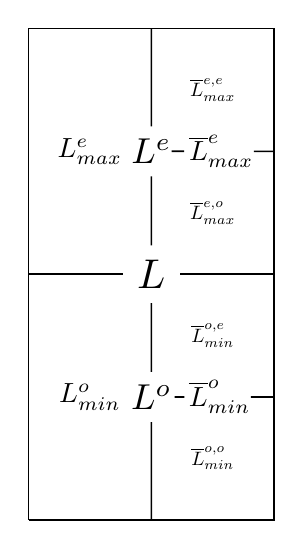
\begin{tikzpicture}[scale = .26]
		\node (L) at (0,0) [scale = 1.5]{$L$};
		\draw [semithick] (-6,0) -- (L) -- (6,0);
		\draw [semithick] (-6,-12) -- (6,-12) -- (6,12) -- (-6,12) -- (-6,-12);
		Statement
		\node (Le) at (0,6) [scale = 1.3] {$L^e$};
		\node (Lemax) at (-3,6) {$ {L}^e_{max}$};
		\node (-Lemax) at (3,6) {$\; \overline{L}^e_{max}$\!\!};
		\node at (3,3) [scale = .7] {$\overline{L}^{e,o}_{max}$};
		\node at (3,9) [scale = .7] {$\overline{L}^{e,e}_{max}$};

		\draw [semithick] (L) -- (Le) -- (0,12);
		\draw [semithick] (6,6) -- (-Lemax) -- (Le);

		\node (Lo) at (0,-6) [scale = 1.3] {$L^o$};
		\node (Lomin) at (-3,-6) {$ {L}^o_{min}$};
		\node (-Lomin) at (3,-6) {$\, \overline{L}^o_{min}$\!\!};
		\node at (3,-3) [scale = .7] {$\overline{L}^{o,e}_{min}$};
		\node at (3,-9) [scale = .7] {$\overline{L}^{o,o}_{min}$};

		\draw [semithick] (L) -- (Lo) -- (0,-12);
		\draw [semithick] (6,-6) -- (-Lomin) -- (Lo);
		\end{tikzpicture}
	\end{center}
\end{minipage}
\ \\

\begin{minipage}{.6\textwidth}
	$R = \big\{ U^0 \ot \bu.U^1 \mid U = \{u_1 < \cdots < u_{q}\} \in \P_q(n), \ \bu \in \overline{U} \big\}$ \vsk
	\begin{tab}
		$R^{e} = \{\ind_{\bu.U}(\bu) = 0\}$ \par \vsk
		\begin{tab}
			$R_{min}^{e} = \{u_q < \bu\}$ \par \vsk
			$\overline{R}_{min}^{e} = R^{e} \setminus R_{min}^{e}$ \vsk
			\begin{tab}
				$\overline{R}_{min}^{e,e} = \{\ind_{\bu.U}(r_{U}^\bu) = 0\}$ \par \vsk
				$\overline{R}_{min}^{e,o} = \{\ind_{\bu.U}(r_{U}^\bu) = 1\}$
			\end{tab}
		\end{tab} \vsk \vsk
		$R^{o} = \{\ind_{\bu.U}(\bu) = 1\}$ \par \vsk
		\begin{tab}
			$R_{max}^{o} = \{\bu < u_1\}$ \par \vsk
			$\overline{R}_{max}^{o} = R^{o} \setminus R_{max}^{o}$ \vsk
			\begin{tab}
				$\overline{R}_{max}^{o,e} = \{\ind_{\bu.U}(l_{U}^\bu) = 0\}$ \par \vsk
				$\overline{R}_{max}^{o,o} = \{\ind_{\bu.U}(l_{U}^\bu) = 1\}$
			\end{tab}
		\end{tab}
	\end{tab}
\end{minipage}
\begin{minipage}{.4\textwidth}
	\begin{center}
		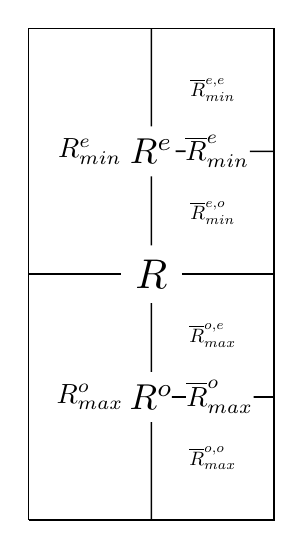
\begin{tikzpicture}[scale = .26]
		\node (L) at (0,0) [scale = 1.5]{$R$};
		\draw [semithick] (-6,0) -- (L) -- (6,0);
		\draw [semithick] (-6,-12) -- (6,-12) -- (6,12) -- (-6,12) -- (-6,-12);

		\node (Le) at (0,6) [scale = 1.3] {$R^e$};
		\node (Lemax) at (-3,6) {$ {R}^e_{min}$};
		\node (-Lemax) at (3,6) {$\overline{R}^e_{min}$\!\!};
		\node at (3,3) [scale = .7] {$\overline{R}^{e,o}_{min}$};
		\node at (3,9) [scale = .7] {$\overline{R}^{e,e}_{min}$};

		\draw [semithick] (L) -- (Le) -- (0,12);
		\draw [semithick] (6,6) -- (-Lemax) -- (Le);

		\node (Lo) at (0,-6) [scale = 1.3] {$R^o$};
		\node (Lomin) at (-3,-6) {$ {R}^o_{max}$};
		\node (-Lomin) at (3,-6) {\,$\overline{R}^o_{max}$\!\!};
		\node at (3,-3) [scale = .7] {$\overline{R}^{o,e}_{max}$};
		\node at (3,-9) [scale = .7] {$\overline{R}^{o,o}_{max}$};

		\draw [semithick] (L) -- (Lo) -- (0,-12);
		\draw [semithick] (6,-6) -- (-Lomin) -- (Lo);
		\end{tikzpicture}
	\end{center} \vsk
\end{minipage}


	With this notation, \eqref{e:big lemma} is equivalent to
	\begin{align*}
	\sum_{L} d_{\bu.U^0} \otimes d_{U^1}\ +\ \
	\sum_{R} d_{U^0} \otimes d_{\bu.U^1} \ & = \
	\sum_{{L}_{max}^{e}} d_{\bu.U^0} \otimes d_{U^1}\ \ +\ \
	\sum_{{R}_{max}^{o}} d_{U^0} \otimes d_{\bu.U^1}\ \\ \ & +\ \
	\sum_{{L}_{min}^{o}} d_{\bu.U^0} \otimes d_{U^1}\ \ +\ \
	\sum_{{R}_{min}^{e}} d_{U^0} \otimes d_{\bu.U^1,}
	\end{align*}
	or, equivalently, to their difference being $0$.
	Explicitly,
	\begin{equation*}
	\sum_{\overline{L}_{max}^{e}} d_{\bu.U^0} \otimes d_{U^1}\ \ +\ \
	\sum_{\overline{R}_{max}^{o}} d_{U^0} \otimes d_{\bu.U^1}\ \ +\ \
	\sum_{\overline{L}_{min}^{o}} d_{\bu.U^0} \otimes d_{U^1}\ \ +\ \
	\sum_{\overline{R}_{min}^{e}} d_{U^0} \otimes d_{\bu.U^1} \ = \ 0,
	\end{equation*}
	which is a direct consequence of the following identities we now prove:
	\begin{equation} \label{e:big lemma four identities}
	\overline{R}_{min}^{e,e} = \overline{L}_{max,}^{e,e} \qquad
	\overline{R}_{min}^{e,o} = \overline{R}_{max,}^{o,e} \qquad
	\overline{L}_{min}^{o,e} = \overline{L}_{max,}^{e,o} \qquad
	\overline{L}_{min}^{o,o} = \overline{R}_{max.}^{o,o}
	\end{equation}

	For a pair $U \in \P_q(n)$ and $\bu \in \overline{U}$ define when possible the sets
	\begin{equation*}
	V^\bu_U = \{v_1 < \cdots < v_q\}, \qquad W_U^\bu = \{w_1 < \cdots < w_q\},
	\end{equation*}
	by
	\begin{align*}
	v_i =
	\begin{cases}
	u_i & \text{ if } u_i \neq l_U^\bu, \\
	\bu	& \text{ if } u_i = l_U^\bu,
	\end{cases}
	\qquad \quad
	w_i =
	\begin{cases}
	u_i & \text{ if } u_i \neq r_U^\bu, \\
	\bu	& \text{ if } u_i = r_U^\bu.
	\end{cases}
	\end{align*}
	Intuitively, $V_U^\bu$ is obtained from $U$ by replacing with $\bu$ the largest element in $U$ that is less than $\bu$.
	A similar description applies to $W_U^\bu$.
	When $U$ and $\bu$ are clear from the context we simplify notation writing $V$ and $W$ instead of $V^\bu_U$ and $W^\bu_U$, and $l$ and $r$ instead of $l_U^\bu$ and $r_U^\bu$.
	Notice that
	\begin{equation*}
	l.V = \bu.U = r.W
	\end{equation*}
	and that for any $u \in \bu.U$ with $u \not \in \{l,\, \bu,\, r\}$ we have
	\begin{equation*}
	\ind_{V}(u) = \ind_{U}(u) = \ind_{W}(u).
	\end{equation*}

	Let us now show that $\overline{R}_{min}^{e,e} = \overline{L}_{max}^{e,e}$.
	Consider $U^0 \otimes \bu.U^1 \in \overline{R}_{min}^{e, e}$ which by definition satisfies $\ind_{\bu.U}(\bu) = \ind_{\bu.U}(l_{U}^\bu) = 0$.
	This is equivalent to $\bu \in V^1$ and $l \in U^0$.
	Therefore,
	\begin{equation*}
	U^0 \otimes \bu.U^1 = \, l.V^0 \otimes V^1
	\end{equation*}
	and, since $l.V^0 \otimes V^1$ is an element in $\overline{L}_{max}^{e,e}$, we have $\overline{R}_{max}^{e,e} \subseteq \overline{L}_{max}^{e,e}$\,.
	Similarly, an element $\bu.U^0 \otimes U^1 \in \overline{L}_{max}^{e,e}$ is equal to $W^0 \otimes r.W^1 \in \overline{R}_{min}^{e,e}$ which gives the other inclusion and proves the first identity in \eqref{e:big lemma four identities}.
	The others are proven analogously, and the lemma follows.
\end{proof}

We can now provide the proof of \cref{l:main} and of our main theorem.

\begin{proof}[Proof of \cref{l:main}]
	For any integer $i$ and $x \in X_n$ we need to prove that
	\begin{equation} \label{e:main thm proof}
	(\partial \circ \Delta_{i} + \Delta_{i} \circ \partial)(x) = (1 + T) \Delta_{i-1}(x).
	\end{equation}
	If $i < 0$ or $i > n+1$ then both sides are equal to $0$ by definition.
	If $i = 0$, the right hand side of \eqref{e:main thm proof} is $0$ by definition and the left hand side is $0$ since the Alexander--Whitney diagonal is a chain map, please consult \cref{ex:alexander-whitney diagonal} for the relationship between $\Delta_0$ and this well known map.
	If $i = n+1$, then the left hand side of \eqref{e:main thm proof} is equal to $0$ by definition and the right hand side is equal to $(1+T) (x \otimes x) = 0$.
	If $i \in \{0, \dots, n-1\}$, \cref{l:boundary of Delta} expresses the left hand side of \eqref{e:main thm proof} as
	\begin{equation*}
	\sum_{\substack{U \in \P_{q}(n) \\ \bu \in \overline{U}}} \Big( d_{\bu.U^0} \otimes d_{U^1} \, + \, d_{U^0} \otimes d_{\bu.U^1} \Big) (x \otimes x),
	\end{equation*}
	whose right hand side is, thanks to \cref{l:big lemma}, equal to $(1+T)\Delta_{i-1}(x)$.
\end{proof}
	
\section{Outlook}

The cup-$i$ products arise from effectively constructing coboundaries that coherently enforce the commutative relation of the cup product in cohomology.
This is part of a general patter in algebraic topology: constructing cochain enforcing cohomological relations lead to further cohomological structures.
In our case, the commutativity relation of cup product gives rise to Steenrod operations.

There are two notable relations satisfied by the Steenrod squares.
The first one, known as the \textit{Cartan relation}, expresses the interaction between these operations and the cup product:
\begin{equation*}
Sq^k \big( [\alpha] [\beta] \big) = \sum_{i+j=k} Sq^i \big([\alpha]\big)\, Sq^j \big([\beta]\big),
\end{equation*}
whereas the second, the \textit{Adem relation} \cite{adem52relations}, expresses dependencies appearing among the iteration of operations:
\begin{equation} \label{equation: adem relations}
Sq^i Sq^j = \sum_{k=0}^{\lfloor i/2 \rfloor} {j-k-1 \choose i-2k} Sq^{i+j-k} Sq^k
\end{equation}
where $\lfloor- \rfloor$ denotes the integer part function and the binomial coefficient is reduced mod-$2$.

To tap into the secondary structure associated with these relations, one needs to provide effective proofs for them, that is to say, construct explicit cochains that enforce the relations when passing to cohomology.
Such effective proofs were recently given respectively in \cite{medina2020cartan} and \cite{medina2020adem}, and we expect the additional structure they unlock will also play a role in applied topology.
	\bibliographystyle{ieeetr}
	\bibliography{bibliography}
\end{document}
